\chapter{Auswertung}
\label{cha:Auswertung}

\section{Untersuchung der Moden mittels Oszilloskop}
Für 3 Moden wurden jeweils Reflektorspannung $U$, Frequenz $f$ und Output Power $U_{out}$ (die Amplitude der Mode) an drei Messstellen gemessen.
Als Messstellen wurden die Maxima und jeweils die Hälften der Maxima links und rechts gewählt.\\
Aus den drei Datenpunkten lassen sich für die Moden selber eine Parabelgleichung aufstellen und für die Frequenzbänder eine kubische Parabel.\\
Die aufgenommen Messwerte lassen sich in \autoref{tab:versuch1} finden. Mithilfe von \textit{python}, den libraries \textit{uncertainties}\cite{uncertainties} und
\textit{matplotlib}\cite{matplotlib} werden die Parameter bestimmt, Ungenauigkeiten berechnet und die Funktionen grafisch dargestellt.\\
Da die meisten Messwerte lediglich abgelesen werden ist hier der systematische Fehler unbekannt und wird im Folgenden vernachlässigt.\\
\begin{table}[htbp] 
    \centering 
    \begin{tabular}{c c c} 
        \toprule $U / \mathrm{V}$ & $U_{out} / \mathrm{mV}$ & $f / \mathrm{GHz}$ \\ 
        \midrule 
        $200$  &  $ 200 $ &  $8,858$ \\
        $211$  &  $ 400 $ &  $8,874$ \\
        $220$  &  $ 200 $ &  $8,886$ \\
        \hline
        $120$  &  $ 185 $ &  $8,854$ \\
        $130$  &  $ 370 $ &  $8,877$ \\
        $140$  &  $ 185 $ &  $8,895 $\\
        \hline
        $70$  &  $ 100 $ &  $8,849$ \\
        $80$  &  $ 200 $ &  $8,881$ \\
        $88$  &  $ 100 $ &  $8,910$ \\
        \bottomrule 
    \end{tabular} 
    \caption[Tabelle]{Positionen der Minima zum Berechnen der Wellenlänge und Frequenz} 
    \label{tab:versuch1} 
\end{table}
In \autoref{fig:moden} sind die gefittet Messwerte mit Ausgleichsfunktionen dargestellt.
\begin{figure}
    \centering
    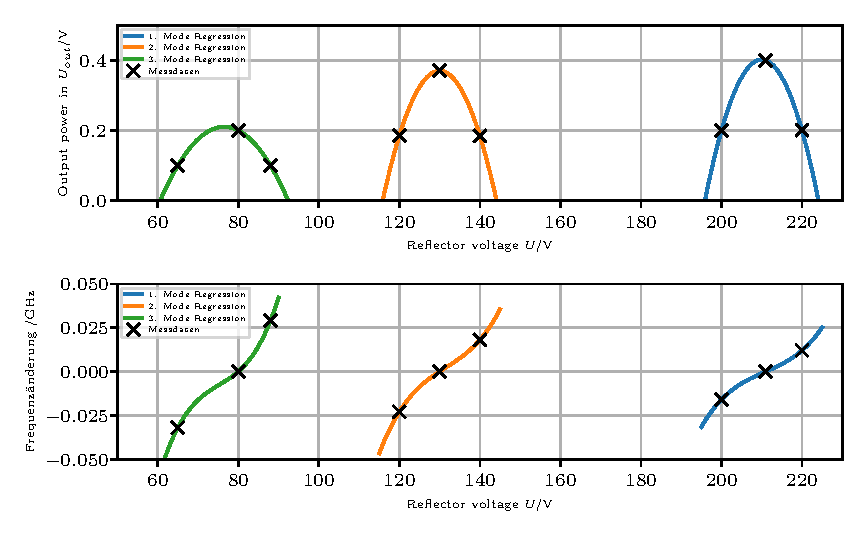
\includegraphics[scale=1]{content/V53_pictures/messung1.pdf}
    \caption{Moden und Frequenzbänder des Klystrons.}
    \label{fig:moden}
\end{figure}

Die Bandbreiten der Moden ergeben sich daher über die Differenz der gemessenen Frequenzen (auf halber Höhe der Maxima) zu:

\begin{align*}
    \Delta f_1 = \qty{0,028}{\giga\hertz} \\
    \Delta f_2 = \qty{0,041}{\giga\hertz} \\
    \Delta f_3 = \qty{0,061}{\giga\hertz}.
\end{align*}

Die elektrische Abstimmempfindlichkeit lässt sich schließlich über 
\begin{align*}
    F_i = \frac{\Delta f_i}{\Delta U_i}
\end{align*}
bestimmen. Wobei $\Delta U_i$ die Differenzen der Reflektorspannungen auf halber Höhe des Maximums sind. Somit ergeben sich folgende Abstimmempfindlichkeiten:\\
\begin{align*}
     F_1 = \qty{1,4}{\mega\hertz\per\volt}\\
     F_2 = \qty{2,05}{\mega\hertz\per\volt}\\
     F_3 = \qty{2,65}{\mega\hertz\per\volt}.
\end{align*}

\section{Frequenzmessung}

Für die direkte Frequenzmessung wird eine Frequenz von
\begin{align*}
    f_1 = \qty{9,103}{\giga\hertz}
\end{align*}
an einem \textit{dip} gemessen.

\section{Wellenlängenmessung}

Der Detektor wurde von einem Minimum in das nächste geschoben und die Positionen als Messwerte $x_1$ und $x_2$ notiert. Diese lassen sich in \autoref{tab:versuch2} finden.\\
Die Hohlleitungswellenlänge $\lambda_g$ berechnet sich aus dem doppelten Abstand des $\Delta x$. Die Frequenz $f_2$ lässt sich anschließend mithilfe von \autoref{eqn:TE01} berechnen.
Das Ergebnis lässt sich ebenfalls in \autoref{tab:versuch2} finden.\\

\begin{table}[htbp] 
    \centering 
    \begin{tabular}{c c c c c} 
        \toprule $x_1 / \mathrm{mm}$ & $x_2 / \mathrm{mm}$ & $\Delta x / \mathrm{mm}$ & $\lambda_g / \mathrm{mm}$ & $f_2 / \mathrm{GHz}$ \\ 
        \midrule 
        $79,1$  &  $104,1$ &  $25$ & $50$ &$ 8,885  \pm 0,01$ \\
        \bottomrule 
    \end{tabular} 
    \caption[Tabelle]{Positionen der Minima zum Berechnen der Wellenlänge und Frequenz} 
    \label{tab:versuch2} 
\end{table}

Mit diesen zwei Messwerten für die Hohlleiterfrequenz lässt sich die Phasengeschwindigkeit $v_{\mathrm{ph}}$ im Hohlleiter bestimmen mittels
\begin{align*}
    v_{\mathrm{ph, i}} = f_i \cdot  \lambda_g
\end{align*}
Somit ergeben sich folgende Phasengeschwindigkeiten:
\begin{align*}
    v_{\mathrm{ph, 1}} = 4,443 \pm 0,005\cdot \, 10^8 \qty{}{\metre\per\second} \\
    v_{\mathrm{ph, 2}} = 4,552 \cdot \, 10^8 \qty{}{\metre\per\second} .
\end{align*}
Der Mittelwert mit Standardabweichung ergibt sich hier zu
\begin{align*}
    v_{\mathrm{ph}} = 4,4970 \pm 0,0024  \cdot \, 10^8 \qty{}{\metre\per\second} .
\end{align*}

\section{Messung der Dämpfung}

In diesem Versuchsabschnitt soll die Herstellerangabe der Dämpfung des Abschwächers überprüft werden. Dafür werden in Abhängigkeit der Tiefe der Millimeterschraube $d$ die Dämpfungen $P$
gemessen. Die Messwerte lassen sich in \autoref{tab:versuch3} finden.\\
\begin{table}[htbp] 
    \centering 
    \begin{tabular}{c  c c c} 
        \toprule $d / \mathrm{mm}$  &  $x_{Herst} / \mathrm{mm}$ & $ P / \mathrm{dB}$ & $ \ln{(P)} / \mathrm{dB}$ \\ 
        \midrule 
        $1$     &   $0,9 $& $2 $ &  $0,69$ \\
        $1,45$  &  $1,4$  & $4 $ & $1,38$ \\
        $1,74$  &  $1,78$ & $6 $ & $1,79$ \\
        $2,01$  &  $2,02$ & $8 $ & $2,08$ \\
        $2,19$  &  $2,22$ & $10$ & $2,30$ \\
        \bottomrule 
    \end{tabular} 
    \caption[Tabelle]{Messwerte der Millimeterschraubenposition und zugehörigen Dämpfungen} 
    \label{tab:versuch3} 
\end{table}
\begin{figure}
    \centering
    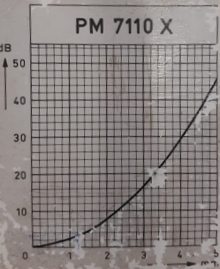
\includegraphics[scale=0.7]{content/V53_pictures/Hersteller.png}
    \caption{Herstellerangaben des Abschwächers.}
    \label{fig:Hersteller}
\end{figure}
Die Angaben des Herstellers des Abschwächers lassen sich auf dem Gerät selber finden. Sie sind außerdem in \autoref{fig:Hersteller} gezeigt. Die Schwächung zeigt einen exponentiellen Verlauf. Es wird
daher der natürliche Logarithmus der Herstellerangaben genommen, linear gefittet und mit den Messwerten verglichen. Der Vergleich ist in \autoref{fig:Dämpf} gezeigt.
\begin{figure}
    \centering
    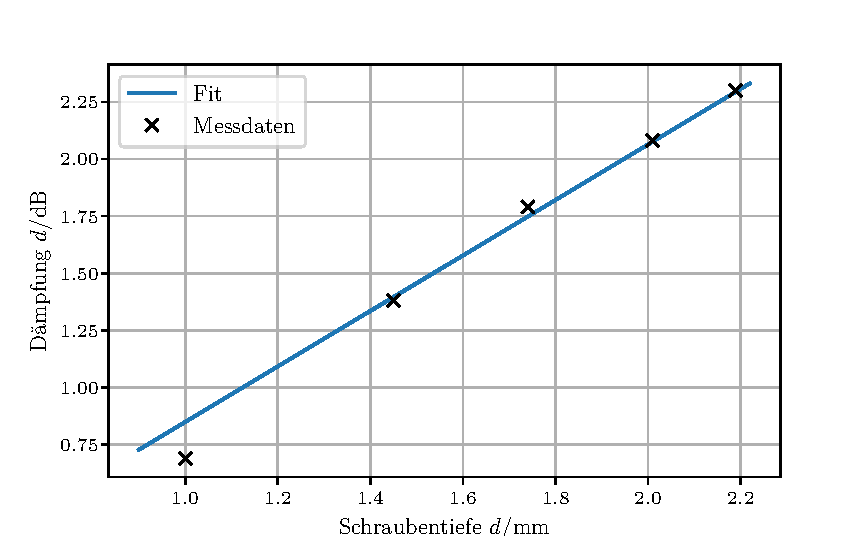
\includegraphics[scale=0.7]{content/V53_pictures/dampfung.pdf}
    \caption{Ausgleichsgerade mithilfe der Herstellerangaben \ref{fig:Hersteller} und die Messwerte.}
    \label{fig:Dämpf}
\end{figure}
Die Abweichung der jeweiligen Messwerte und der Angaben des Herrstellers sind im Durchschnitt $4 \%$.
\section{Messung des Stehwellenverhältnisses}
Es werden im folgenden drei Methoden zur Messung des Stehwellenverhältnisses evaluiert.
\subsection{Direkte Methode}

Die direkte Methode wird über das SWR-Meter gemessen. Hier wird bei verschiedenen Tiefen der Störstelle $d$ der Ausschlag am SWR-Meter gemessen. Die Messwerte befinden sich in \autoref{tab:Direkt}.
\begin{table}[htbp] 
    \centering 
    \begin{tabular}{c  c} 
        \toprule $d / \mathrm{mm}$  &  SWR  \\ 
        \midrule 
        $0$  &  $1,21$ \\
        $1$  &  $1,24$ \\
        $2$  &  $1,26$\\
        $3$  &  $1,3$\\
        $4$  &  $1,36$\\
        $5$  &  $1,51$\\
        $6$  &  $1,8$\\
        $7$  &  $2,2$\\
        $8$  &  $2,3$\\
        $9$  &  $\infty$\\
        \bottomrule 
    \end{tabular} 
    \caption[Tabelle]{Messwerte der Millimeterschraubenposition der Störstelle und das Stehwellenverhältniss} 
    \label{tab:Direkt} 
\end{table}

\subsection{$\qty{3}{\decibel}$-Methode}

Es werden Vollausschläge links und rechts eines Minimas gesucht. Die Messwerte lassen sich in \autoref{tab:3db} finden. Die Wellenlänge wurde bereits berechnet.
\begin{table}[htbp] 
    \centering 
    \begin{tabular}{c  c c c} 
        \toprule $d_1 / \mathrm{mm}$ & $d_2 / \mathrm{mm}$ &  $\lambda_g  / \mathrm{mm}$ & $S$\\ 
        \midrule 
        $83,0$ &  $84,3$ & $50$ & $12,24$ \\
        \bottomrule 
    \end{tabular} 
    \caption[Tabelle]{Messwerte zur $\qty{3}{\decibel}$-Methode} 
    \label{tab:3db} 
\end{table}
Zur Berechnung des Stehwellenverhältnis $S$ wird \autoref{eqn:S_3dB_easy} verwendet. Die Ergebnisse lassen sich ebenfalls in \autoref{tab:3db} finden.

\subsection{Abschwächer-Methode}

Die zwei gemessenen Dämpfungen sind in \autoref{tab:Abschw} zu finden. Das Stehwellenverhältnis $S$ wird über \autoref{eqn:S_abschwaecher} berechnet und ist 
ebenfalls in der Tabelle zu finden.
\begin{table}[htbp] 
    \centering 
    \begin{tabular}{c  c c} 
        \toprule $A_1 / \mathrm{dB}$ & $A_2 / \mathrm{dB}$ & $S$\\ 
        \midrule 
        $20$ &  $5$ & $5,62$ \\
        \bottomrule 
    \end{tabular} 
    \caption[Tabelle]{Messwerte der Dämpfungen} 
    \label{tab:Abschw} 
\end{table}